\documentclass{amsart}
\usepackage{amsaddr}
\usepackage{amssymb}
\usepackage[latin1]{inputenc}
\usepackage[swedish,english]{babel}
\usepackage{ifpdf}
\ifpdf
\usepackage[pdftex]{graphicx}
\usepackage{epstopdf}
\else
\usepackage[dvips]{graphicx}
\fi
% \usepackage{subfigure}
% \usepackage{sidecap}
\usepackage[pdftitle={The Bayesian Approach to Inverse Problems},
pdfauthor={Robin Eriksson},
pdffitwindow=true,
breaklinks=true,
colorlinks=true,
urlcolor=blue,
linkcolor=red,
citecolor=red,
anchorcolor=red]{hyperref}
% \usepackage{pdfpages}
\usepackage{algorithm}
% \usepackage{algorithmic}
\usepackage[noend]{algpseudocode}
\usepackage{dsfont}
\usepackage[numbers,sort&compress]{natbib}
\usepackage{appendix}
\usepackage[section]{placeins}
% **************************************************************************
\usepackage[margin=1.25in]{geometry}
\usepackage{subcaption}
% ***************************************************************************
\usepackage{microtype}
\usepackage{parskip}

\usepackage{listings}
\usepackage{color} %red, green, blue, yellow, cyan, magenta, black, white
\definecolor{mygreen}{RGB}{28,172,0} % color values Red, Green, Blue
\definecolor{mylilas}{RGB}{170,55,241}

\usepackage{mathtools}
% ***************************************************************************
\numberwithin{equation}{section}
\numberwithin{table}{section}
\numberwithin{figure}{section}

\theoremstyle{plain}
\newtheorem{theorem}{Theorem}[section]
\newtheorem{lemma}[theorem]{Lemma}
\newtheorem{proposition}[theorem]{Proposition}
\newtheorem{corollary}[theorem]{Corollary}
\newtheorem{conjecture}[theorem]{Conjecture}
% \newtheorem{algorithm}[theorem]{Algorithm}
% \newtheorem{criterion}[theorem]{Criterion}

\theoremstyle{definition}
\newtheorem{definition}{Definition}[section]
\newtheorem{assumption}[definition]{Assumption}
\newtheorem{convention}[definition]{Convention}
\newtheorem{example}[definition]{Example}
% \newtheorem{problem}[definition]{Problem}

\theoremstyle{remark}
\newtheorem*{remark}{Remark}
% \newtheorem*{note}{Note}
% \newtheorem*{notation}{Notation}
% \newtheorem*{summary}{Summary}
% \newtheorem{theorem}{Theorem}[section]
% \newtheorem{lemma}[theorem]{Lemma}

\renewcommand{\Pr}{\mathbf{P}}
\renewcommand{\P}{P}

% *** use these commands to write comments; they are easy to spot in the text!
\newcommand{\comment}[1]{\textcolor{blue}{\{#1\}}}
\newcommand{\margincomment}[1]{* \marginpar{\textcolor{blue}{*\{#1\}}}}


% *** todo list! ***
\usepackage{enumitem,amssymb}
\newlist{todolist}{itemize}{2}
\setlist[todolist]{label=$\square$}
\usepackage{pifont}
\newcommand{\cmark}{\ding{51}}%
\newcommand{\xmark}{\ding{55}}%
\newcommand{\done}{\rlap{$\square$}{\raisebox{2pt}{\large\hspace{1pt}\cmark}}%
  \hspace{-2.5pt}}
\newcommand{\wontfix}{\rlap{$\square$}{\large\hspace{1pt}\textcolor{red}{\xmark}}}

% **************************************************************************

\begin{document}

\lstset{language=Matlab,%
  % basicstyle=\color{red},
  breaklines=true,%
  morekeywords={matlab2tikz},
  keywordstyle=\color{blue},%
  morekeywords=[2]{1}, keywordstyle=[2]{\color{black}},
  identifierstyle=\color{black},%
  stringstyle=\color{mylilas},
  commentstyle=\color{mygreen},%
  showstringspaces=false,%without this there will be a symbol in the places where there is a space
  numbers=left,%
  numberstyle={\tiny \color{black}},% size of the numbers
  numbersep=9pt, % this defines how far the numbers are from the text
  emph=[1]{for,end,break},emphstyle=[1]\color{red}, %some words to emphasise
  % emph=[2]{word1,word2}, emphstyle=[2]{style},
  frame = single
}

\title[]{BAIP -- The model problem}

\author[R. Eriksson]{Robin Eriksson}
\email{\href{mailto:robin.eriksson@it.uu.se}{robin.eriksson@it.uu.se}}
% \address{Division of Scientific Computing \\
% Department of Information Technology \\
% Uppsala University \\
% SE-751 05 Uppsala, Sweden.}

% \subjclass[2010]{Primary: NNXMM; Secondary: NNXMM}

% \keywords{}

\date{\today}


\selectlanguage{english}

\maketitle

% **************************************************************************
\section{Introduction}
Consider the model problem
\begin{equation}
  \label{eq:model}
  y' = \lambda y,\quad y(0) = 1,
\end{equation}
with observations
\begin{equation}
  \label{eq:observations}
  z_i = y(t_i) + \mathcal{N}(0,\sigma).
\end{equation}
The one unknown is $\lambda$. Try to generalize to the situation where
one is only able to compute the solution to some other approximate
solution,
\begin{equation}
  \label{eq:apsol}
  w' = \lambda_{\Delta t} w,\quad w(0) = 1,
\end{equation}
where $\lambda_{\Delta t} \to \lambda$ as $\Delta t \to 0$.

\begin{itemize}
\item Suppose the cost of one trajectory is $\sim 1/\Delta t$, what is
  then the cost to obtain $|\hat{y}-y| < \text{TOL}$?
\end{itemize}

\subsection{A guess}
$\text{error} \sim \frac{1}{\sqrt{N_{\text{data}}}} + \Delta t \sim \text{TOL}$,
  assume optimal to balance the terms (?), then
  $N_\text{data} \sim 1/\Delta t^2$. Cost $\dots$ perhaps
  $N_{\text{data}} \frac{1}{\Delta t}$ for one likelihood (?), then
  $\text{cost} \sim \frac{1}{\text{TOL}^3}$. However this ignores the
number of evaluations in an optimizer routine or the number of
posterior samples from an MCMC to compute the estimator $\dots$

\section{The Bayes' inversion checklist}
\begin{itemize}
\item Define a suitable prior measurement $\mu_0$ and noise measure
  $\mathbb{Q}_0$ whose independent product form the reference measure $\nu_0$.
\item Determine the potential $\Phi$ such that formula (3.3) holds.
\item Show that $\Phi$ is $\nu_0$ measurable.
\item Show that the normalization constant $Z$ given (3.5) is positive
  almost surely with respect to $y \sim \mathbb{Q}_0$.
\end{itemize}

\section{A todo approach}
A list:
\begin{todolist}
\item[\done] Write code for a super simple example, and output a
  plot. Consider a point-estimate of $\lambda$, i.e., 1 value, and
  generate $N_{\text{data}}$ realisations of $z$. How does the
  ribbon-plot ($\text{{\it mean}} \pm 2 \times \text{{\it sd}}$) look?
  \begin{itemize}
  \item See \verb;/CODE/modelExplore.ipynb; for the code

    \begin{figure}[H]
      \centering
      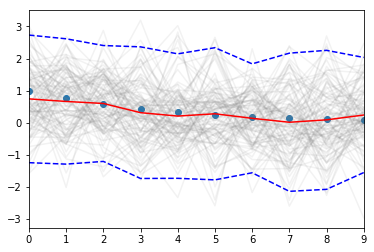
\includegraphics[width=0.5\textwidth]{CODE/ribbon.png}
      \caption{Simple test with $\lambda = -2.5$, one underlying truth
        (dots), 100 noisy obserations (grey), the mean of observations
        (red), and $\pm 2$ sd (dashed blue).}
    \end{figure}
  \end{itemize}


\item Follow the checklist on the ``simple'' model. Assume no discretization.
\item Now, assume $\Delta t$ discretization, where
  $\lambda_{\Delta t} \rightarrow \lambda$ as $\Delta t \rightarrow 0$.
\item What is the cost to obtain \verb;error < TOL;?
  \begin{itemize}
  \item True $\lambda = -2.5$. If we use the same observation, but
    exlude increasingly many data points. The error increase as in the figure below.
    \begin{figure}[H]
      \centering
      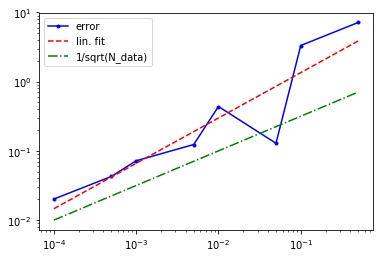
\includegraphics[width=0.5\textwidth]{CODE/errorplot.png}
      \caption{error (blue), polyfit (red), $1/\sqrt(N_{\text{data}}$) (green)}
    \end{figure}

     \begin{figure}[H]
      \centering
      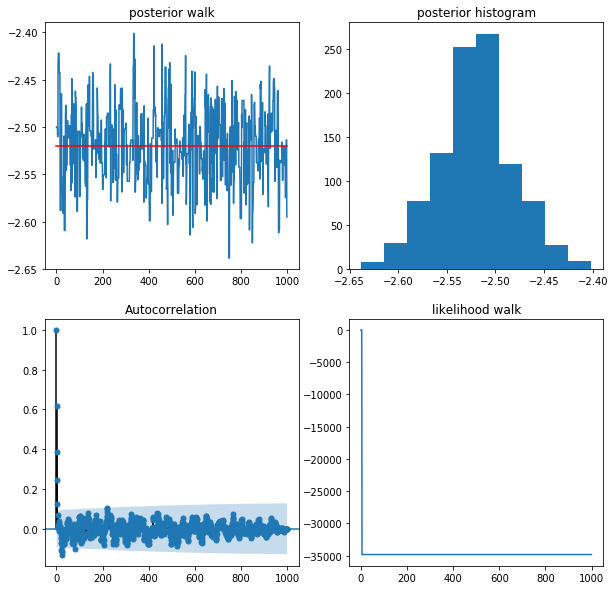
\includegraphics[width=0.8\textwidth]{CODE/mcmcoutput.png}
      \caption{output from the MCMC algo at the smallest $\Delta_t$}
    \end{figure}
  \end{itemize}

\end{todolist}

Additional notes:
\begin{itemize}
\item In the previous chapters in the book, they never really talk about data. Look into that.
\end{itemize}



\end{document}
